% =====================================================================
% Artigo SBC — Análise de segurança de repositórios Java da NSA
% Template oficial da SBC (sbc-template). Ver Artigo/README.md para
% instruções de compilação no Overleaf.
% =====================================================================
\documentclass[12pt]{article}

\usepackage{sbc-template}
\usepackage{graphicx,url}
\usepackage[utf8]{inputenc}
\usepackage[brazil]{babel}
\usepackage{booktabs}
\usepackage{multirow}

\sloppy

\title{Métricas de qualidade de código predizem arquivos Java propensos a
risco de segurança? Um estudo empírico em repositórios da \textit{National
Security Agency} sob a ótica da ISO/IEC~25010}

\author{Igor Mariano\inst{1}}

\address{Curso de Engenharia de Software\\
  \email{igor.mariano@envoylog.com.br}
}

\begin{document}

\maketitle

\begin{resumo}
Investiga-se, por análise estática (apenas clone, sem \textit{build}), se
métricas de qualidade de código predizem arquivos Java propensos a risco de
segurança. Foram analisados 10 repositórios Java da organização
\textit{NationalSecurityAgency} (29.662 arquivos \texttt{.java}), construindo-se
um \textit{dataset} em nível de arquivo cujo rótulo provém de um analisador SAST
(Semgrep) e cujas \textit{features} vêm de métricas de
manutenibilidade/processo (complexidade, métricas OO~CK e métricas de
histórico), mapeadas à característica \emph{Segurança} do modelo de qualidade
ISO/IEC~25010. Cinco modelos foram avaliados com \textit{GroupKFold} por
repositório. Os resultados (ROC-AUC até 0,82) indicam que tais métricas
carregam sinal discriminante, ainda que a classificação precisa seja limitada
pelo forte desbalanceamento (0,53\% de positivos).
\end{resumo}

\begin{abstract}
We investigate, through static analysis (clone-only, no build), whether code
quality metrics can predict Java files prone to security risk. We analysed 10
Java repositories from the \textit{NationalSecurityAgency} organisation (29,662
\texttt{.java} files), building a file-level dataset whose label comes from a
SAST tool (Semgrep) and whose features come from maintainability/process
metrics (complexity, CK OO metrics and history metrics), mapped to the
\emph{Security} characteristic of the ISO/IEC~25010 quality model. Five models
were evaluated with repository-wise \textit{GroupKFold}. Results (ROC-AUC up to
0.82) indicate that such metrics carry discriminant signal, although precise
classification is limited by the strong class imbalance (0.53\% positives).
\end{abstract}

% =====================================================================
\section{Introdução}
% =====================================================================

A garantia de segurança em sistemas de software é um requisito crítico, e a
identificação antecipada de artefatos propensos a falhas de segurança permite
direcionar esforços de revisão e teste. A norma \textbf{ISO/IEC~25010}
\cite{iso25010} estabelece um modelo de qualidade de produto no qual
\emph{Segurança} é uma característica de primeira ordem, ao lado de
\emph{Manutenibilidade} e \emph{Confiabilidade}. Uma questão de pesquisa
recorrente em Mineração de Repositórios de Software (MSR) é se medidas associadas
a uma característica de qualidade ajudam a prever fragilidades em outra
\cite{shin2011,zimmermann2010}.

Este trabalho testa empiricamente a seguinte pergunta:

\begin{quote}
\textit{Métricas de qualidade de código (complexidade, métricas orientadas a
objetos e métricas de processo) são capazes de predizer arquivos Java propensos
a riscos de segurança?}
\end{quote}

A leitura normativa é direta: trata-se de verificar se medidas de
\emph{Manutenibilidade}/\emph{Confiabilidade} (definidas pela
ISO/IEC~25023~\cite{iso25023}) predizem fraquezas na característica
\emph{Segurança} do modelo ISO/IEC~25010. As contribuições são: (i)~um
\textit{dataset} reprodutível em nível de arquivo \texttt{.java} para 10
sistemas Java reais; (ii)~um \textit{pipeline} de coleta estática e de
\textit{Machine Learning} sem necessidade de \textit{build}; e (iii)~evidência
sobre o poder preditivo das métricas de qualidade quanto a risco de segurança,
discutida à luz da ISO/IEC~25010.

% =====================================================================
\section{Fundamentação Teórica}
% =====================================================================

\subsection{A série SQuaRE e a ISO/IEC 25010}
A família \textbf{ISO/IEC~25000} (SQuaRE --- \textit{Software Quality
Requirements and Evaluation}) organiza as normas de qualidade de software
\cite{iso25000}. A \textbf{ISO/IEC~25010} \cite{iso25010} define o \emph{modelo}
de qualidade do produto; na versão de 2011, possui oito características, entre
elas \emph{Segurança}, decomposta em cinco sub-características:
\emph{Confidencialidade}, \emph{Integridade}, \emph{Não-repúdio},
\emph{Responsabilização} e \emph{Autenticidade}. A revisão de 2023 adicionou
\emph{Safety} como característica própria e a sub-característica
\emph{Resistência} à Segurança. A \textbf{ISO/IEC~25023} \cite{iso25023}
define as \emph{medidas} das características --- é a norma que fundamenta
\emph{como} medir. O modelo (25010) e as medidas (25023) são citados em conjunto.

\subsection{Análise estática: SAST e SCA}
\emph{Static Application Security Testing} (SAST) analisa o código-fonte em
busca de fraquezas (ex.: injeção, desserialização insegura). \emph{Software
Composition Analysis} (SCA) examina dependências declaradas em busca de
vulnerabilidades conhecidas (CVE). Ambas operam sem executar o sistema.

\subsection{Métricas de qualidade}
A complexidade ciclomática \cite{mccabe1976} mede o número de caminhos
independentes em um método. As métricas orientadas a objetos de Chidamber e
Kemerer \cite{ck1994} --- WMC, DIT, CBO, RFC, LCOM --- capturam acoplamento,
coesão e herança. Métricas de processo (número de \textit{commits}, autores
distintos, \textit{churn}, idade do arquivo) capturam a dinâmica de evolução
\cite{spadini2018}.

\subsection{Trabalhos relacionados}
A predição de defeitos e de vulnerabilidades a partir de métricas de código é
amplamente estudada. \citeonline{shin2011} avaliaram complexidade, \textit{code
churn} e atividade de desenvolvedores como indicadores de vulnerabilidades.
\citeonline{zimmermann2010} predisseram vulnerabilidades no Windows~Vista.
\citeonline{walden2014} compararam métricas de software e \textit{text mining}
para prever componentes vulneráveis. Este trabalho difere ao amarrar
explicitamente as \textit{features} às sub-características da ISO/IEC~25010 e ao
adotar uma abordagem 100\% estática (sem \textit{build}).

% =====================================================================
\section{Metodologia}
% =====================================================================

\subsection{Seleção dos repositórios}
Selecionaram-se 10 repositórios Java da organização
\textit{NationalSecurityAgency} (Tabela~\ref{tab:repos}), priorizando sistemas
substanciais e descartando módulos triviais. \textbf{Transparência:} quatro
repositórios (\texttt{datawave}, \texttt{datawave-query-service},
\texttt{datawave-audit-service}, \texttt{datawave-authorization-service})
pertencem ao mesmo ecossistema \emph{DataWave}, o que constitui variável de
confusão e limitação de validade externa.

\subsection{Abordagem estática (apenas clone, sem \textit{build})}
Os repositórios foram \textbf{apenas clonados}; nenhum projeto foi compilado ou
executado. Toda a \textit{stack} opera sobre o código-fonte e o histórico Git.

\subsection{\textit{Pipeline} de extração}
Adotou-se uma ferramenta canônica por dimensão, evitando dupla contagem
(Tabela~\ref{tab:stack}):
\begin{itemize}
  \item \textbf{Alvo (SAST):} Semgrep (\texttt{--config auto}), que rotula cada
  arquivo \texttt{.java} com \texttt{has\_security\_risk}~$=1$ se houver
  $\geq 1$ achado de segurança;
  \item \textbf{\textit{Features} de qualidade:} complexidade (lizard),
  estrutura/OO (javalang), métricas CK (WMC, DIT, CBO, RFC, LCOM) e métricas de
  processo (PyDriller);
  \item \textbf{Descritivo:} OSV (SCA de dependências) e detect-secrets
  (segredos).
\end{itemize}

\begin{table}[ht]
\centering
\caption{Mapeamento ferramenta $\rightarrow$ dimensão $\rightarrow$ ISO/IEC 25010.}
\label{tab:stack}
\small
\begin{tabular}{@{}lll@{}}
\toprule
\textbf{Dimensão} & \textbf{Ferramenta} & \textbf{ISO/IEC 25010} \\
\midrule
SAST (alvo)       & Semgrep        & Segurança (Integ./Confid./Autent.) \\
Complexidade      & lizard         & Manutenibilidade \\
Estrutura/OO      & javalang, CK   & Manutenibilidade/Confiabilidade \\
Processo          & PyDriller      & Manutenibilidade \\
SCA (descritivo)  & OSV            & Segurança $>$ Resistência \\
Segredos (descr.) & detect-secrets & Segurança $>$ Confidencialidade \\
\bottomrule
\end{tabular}
\end{table}

\subsection{Construção do \textit{dataset}}
A unidade de análise é o arquivo \texttt{.java}. Consolidaram-se, por arquivo,
o rótulo de segurança (Semgrep) e as \textit{features} de qualidade/processo,
totalizando \textbf{29.662 arquivos} e 32 \textit{features}.

\subsection{Prevenção de vazamento e desbalanceamento}
Para evitar circularidade, \textbf{nenhuma \textit{feature} deriva do alvo}: as
entradas vêm exclusivamente de manutenibilidade, OO e processo --- dimensões
distintas da que origina o rótulo. Como arquivos com risco são raros (0,53\%),
a avaliação é liderada por \textbf{Precision, Recall, F1 e ROC-AUC} (não
\textit{accuracy}); o desbalanceamento é tratado com
\texttt{class\_weight="balanced"} e SMOTE \cite{smote2002} nos
\textit{folds} de treino.

\subsection{Validação e modelos}
Usou-se \textbf{GroupKFold} agrupado por repositório, treinando em $N-1$
repositórios e testando no restante, para medir generalização entre projetos.
\textit{Folds} de teste de classe única são descartados de forma robusta.
Comparam-se: Regressão Logística, Árvore de Decisão, \textit{Random Forest}
\cite{breiman2001}, \textit{XGBoost} \cite{xgboost2016} e \textit{LightGBM}. A
importância de \textit{features} é reportada pelo \textit{Random Forest} (Gini)
e por SHAP \cite{shap2017}.

% =====================================================================
\section{Resultados e Discussão}
% =====================================================================

\subsection{Postura de segurança dos repositórios}
A Tabela~\ref{tab:repos} resume a postura por repositório (valores brutos e
normalizados por KLOC). A Figura~\ref{fig:kloc} mostra que repositórios menores
de pesquisa (\texttt{fractalrabbit}, \texttt{rank-based-linkage}) apresentam
\emph{maior densidade} de achados por KLOC, enquanto o \texttt{ghidra},
embora concentre o maior número absoluto de achados (275), tem baixa densidade.

\begin{table}[ht]
\centering
\caption{Postura de segurança por repositório (Semgrep, OSV, segredos).}
\label{tab:repos}
\scriptsize
\begin{tabular}{@{}lrrrrrr@{}}
\toprule
\textbf{Repositório} & \textbf{Arq.\ Java} & \textbf{KLOC} & \textbf{Achados} &
\textbf{/KLOC} & \textbf{CVEs} & \textbf{Segredos} \\
\midrule
ghidra                         & 15589 & 2046.2 & 275 & 0.13 & 0  & 0   \\
datawave                       & 4302  & 565.9  & 173 & 0.31 & 30 & 191 \\
timely                         & 359   & 31.1   & 20  & 0.64 & 1  & 16  \\
emissary                       & 676   & 67.4   & 12  & 0.18 & 0  & 33  \\
lemongrenade                   & 110   & 13.9   & 5   & 0.36 & 9  & 1   \\
datawave-query-service         & 54    & 14.0   & 5   & 0.36 & 0  & 2   \\
rank-based-linkage             & 34    & 1.6    & 3   & 1.82 & 0  & 0   \\
fractalrabbit                  & 31    & 1.1    & 3   & 2.72 & 0  & 0   \\
datawave-audit-service         & 48    & 7.7    & 1   & 0.13 & 0  & 3   \\
datawave-authorization-service & 51    & 3.5    & 1   & 0.29 & 0  & 5   \\
\bottomrule
\end{tabular}
\end{table}

\begin{figure}[ht]
\centering
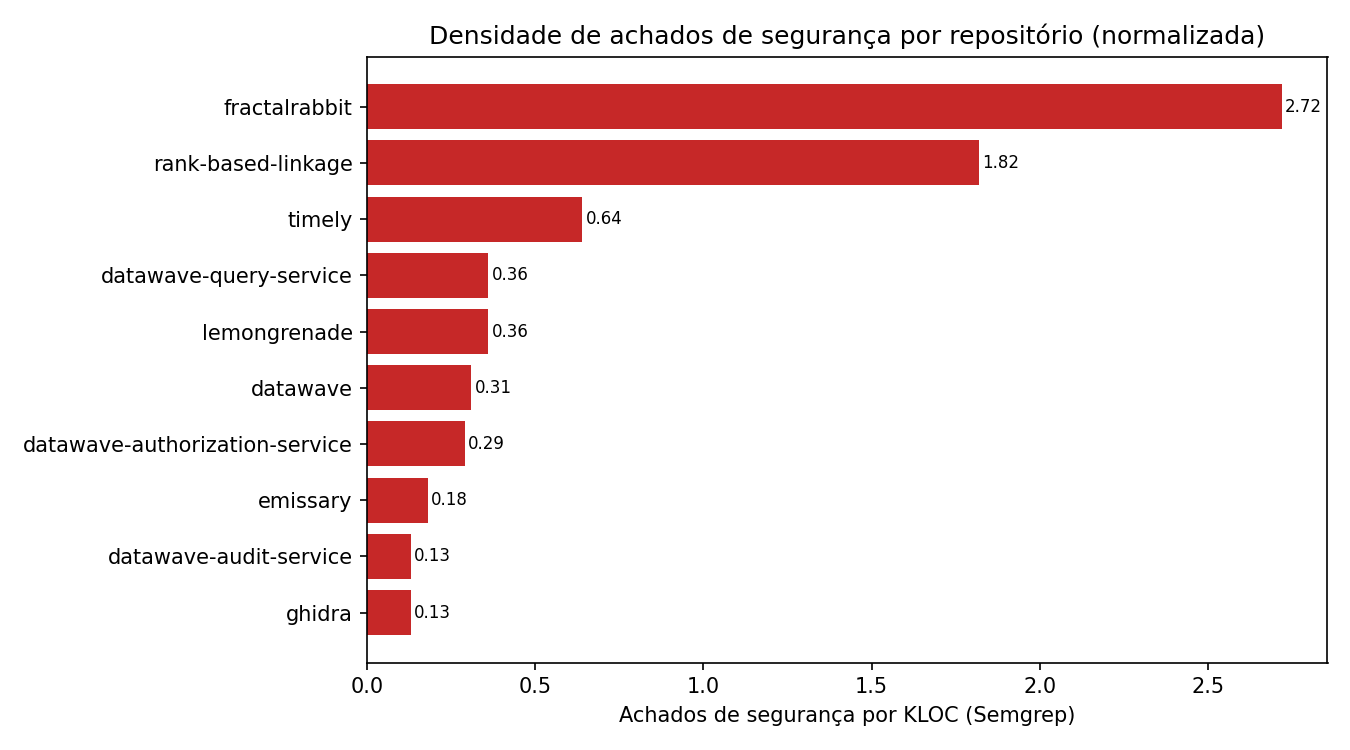
\includegraphics[width=0.85\textwidth]{figuras/security_per_kloc.png}
\caption{Densidade de achados de segurança por KLOC (Semgrep).}
\label{fig:kloc}
\end{figure}

\subsection{Mapeamento às sub-características da Segurança (25010)}
A Figura~\ref{fig:cwe} e a Tabela~\ref{tab:subchar} relacionam os achados às
sub-características. Predominam \emph{Integridade} (276 achados; CWE-470 reflexão
insegura, CWE-89 injeção SQL, CWE-78 injeção de comando, CWE-502
desserialização) e \emph{Confidencialidade} (117; CWE-319 transmissão em texto
claro, criptografia fraca). \emph{Autenticidade} aparece de forma minoritária
(11; CWE-295 validação de certificado, CWE-798 credenciais embutidas).
\emph{Resistência} é evidenciada por 40 CVEs em dependências diretas (OSV).
\emph{Não-repúdio} e \emph{Responsabilização} não são mensuráveis estaticamente
e são tratados como discussão qualitativa.

\begin{table}[ht]
\centering
\caption{Cobertura das sub-características de Segurança (ISO/IEC 25010).}
\label{tab:subchar}
\small
\begin{tabular}{@{}lrl@{}}
\toprule
\textbf{Sub-característica} & \textbf{Evidências} & \textbf{Fonte} \\
\midrule
Integridade        & 276 & Semgrep \\
Confidencialidade  & 117 & Semgrep \\
Autenticidade      & 11  & Semgrep \\
Resistência (2023) & 40  & OSV (dependências) \\
Não classificada   & 94  & Semgrep \\
\bottomrule
\end{tabular}
\end{table}

\begin{figure}[ht]
\centering
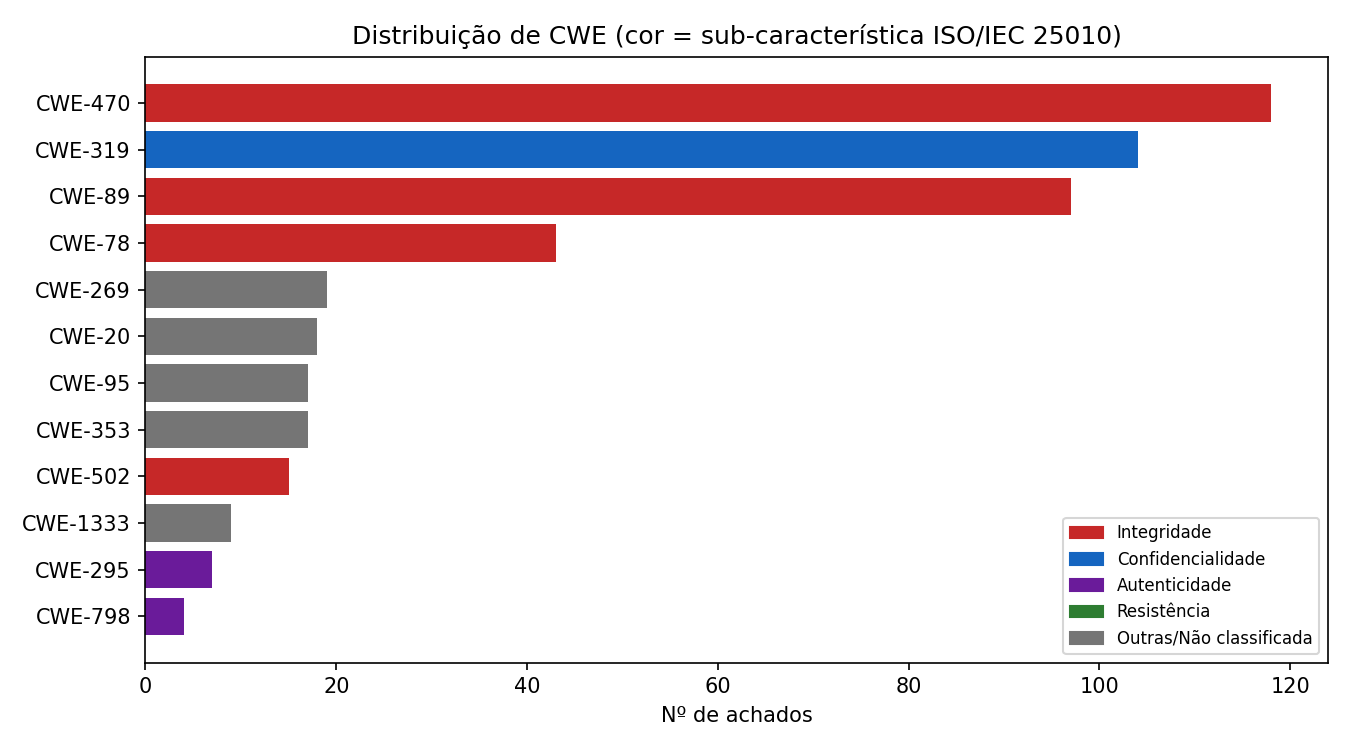
\includegraphics[width=0.85\textwidth]{figuras/cwe_distribution.png}
\caption{Distribuição de CWE colorida por sub-característica da ISO/IEC 25010.}
\label{fig:cwe}
\end{figure}

\subsection{Comparação dos modelos}
A Tabela~\ref{tab:ml} e a Figura~\ref{fig:roc} apresentam os resultados sob
\textit{GroupKFold}. Os modelos atingem \textbf{ROC-AUC entre 0,66 e 0,82},
indicando que as métricas de qualidade ordenam arquivos arriscados acima da
média --- isto é, carregam sinal discriminante. Contudo, Precision/Recall/F1
são baixos: a Regressão Logística (com pesos balanceados) alcança o melhor
\textbf{Recall (0,69)} ao custo de muitos falsos positivos, enquanto os modelos
de árvore quase não predizem positivos no limiar padrão. Esse contraste é
esperado sob desbalanceamento extremo (0,53\%) e reforça a escolha de liderar a
avaliação por ROC-AUC e Recall em vez de \textit{accuracy}.

\begin{table}[ht]
\centering
\caption{Desempenho médio por modelo (GroupKFold por repositório).}
\label{tab:ml}
\small
\begin{tabular}{@{}lrrrr@{}}
\toprule
\textbf{Modelo} & \textbf{Precision} & \textbf{Recall} & \textbf{F1} & \textbf{ROC-AUC} \\
\midrule
Regressão Logística & 0.031 & \textbf{0.691} & 0.059 & 0.811 \\
Árvore de Decisão   & 0.032 & 0.258 & 0.056 & 0.657 \\
\textit{Random Forest} & 0.003 & 0.004 & 0.003 & \textbf{0.817} \\
XGBoost             & 0.000 & 0.000 & 0.000 & 0.776 \\
LightGBM            & 0.003 & 0.004 & 0.004 & 0.803 \\
\bottomrule
\end{tabular}
\end{table}

\begin{figure}[ht]
\centering
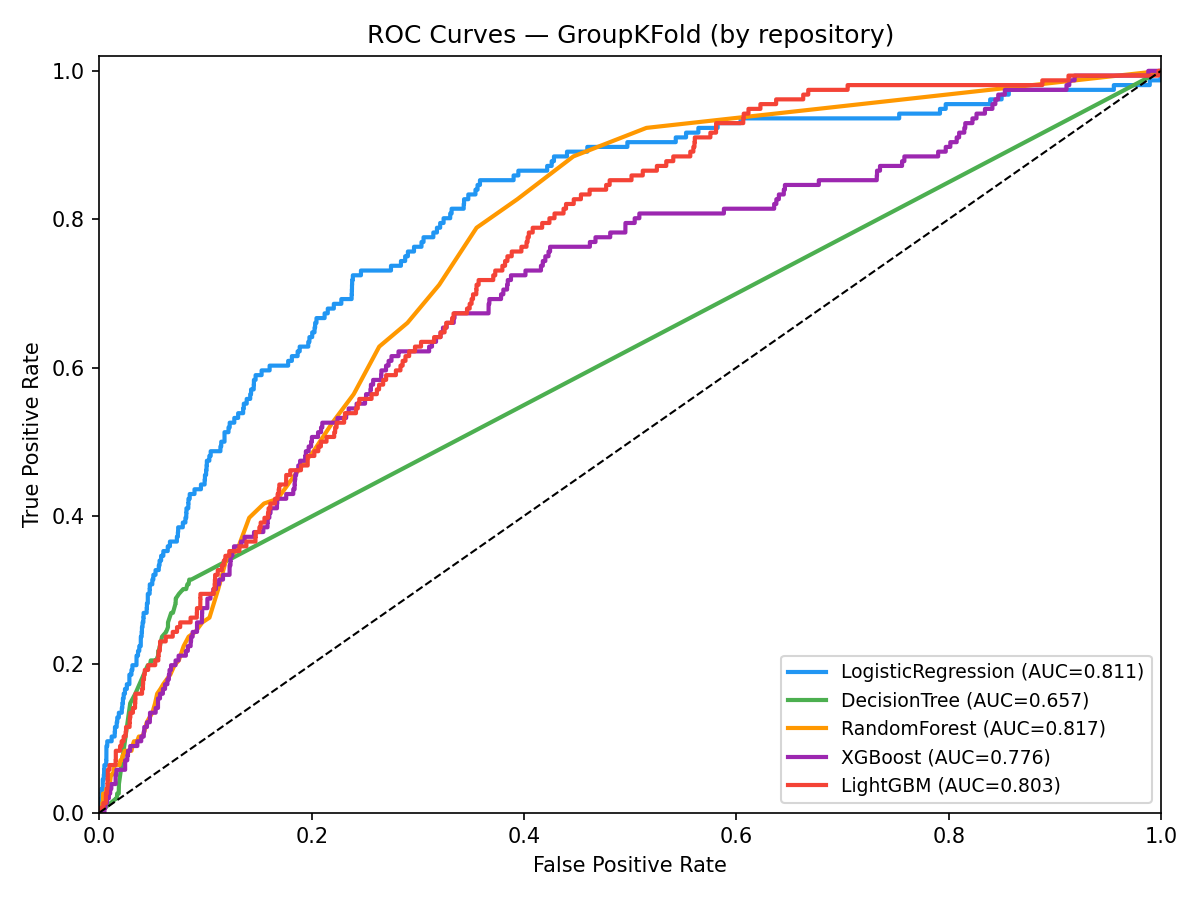
\includegraphics[width=0.8\textwidth]{figuras/roc_curves.png}
\caption{Curvas ROC dos cinco modelos (validação GroupKFold por repositório).}
\label{fig:roc}
\end{figure}

\subsection{Importância das \textit{features} e leitura à luz da ISO/IEC 25010}
A Figura~\ref{fig:imp} mostra a importância (Gini) do \textit{Random Forest}. As
\textit{features} mais preditivas são de \textbf{complexidade}
(\texttt{ccn\_mean}, \texttt{ccn\_max}, \texttt{ccn\_sum}), \textbf{tamanho}
(\texttt{tokens\_sum}, \texttt{nloc\_sum}), \textbf{acoplamento/coesão OO}
(\texttt{rfc}, \texttt{wmc}) e \textbf{processo} (\texttt{days\_since\_change},
\texttt{file\_age\_days}). Esse ranking sustenta o argumento central do estudo:
medidas de \emph{Manutenibilidade} e \emph{Confiabilidade} (no vocabulário da
ISO/IEC~25010) são as que mais se associam à propensão a risco de
\emph{Segurança} --- ou seja, arquivos grandes, complexos e fortemente acoplados
tendem a concentrar achados de segurança, em linha com a literatura de predição
de vulnerabilidades \cite{shin2011,walden2014}.

\begin{figure}[ht]
\centering
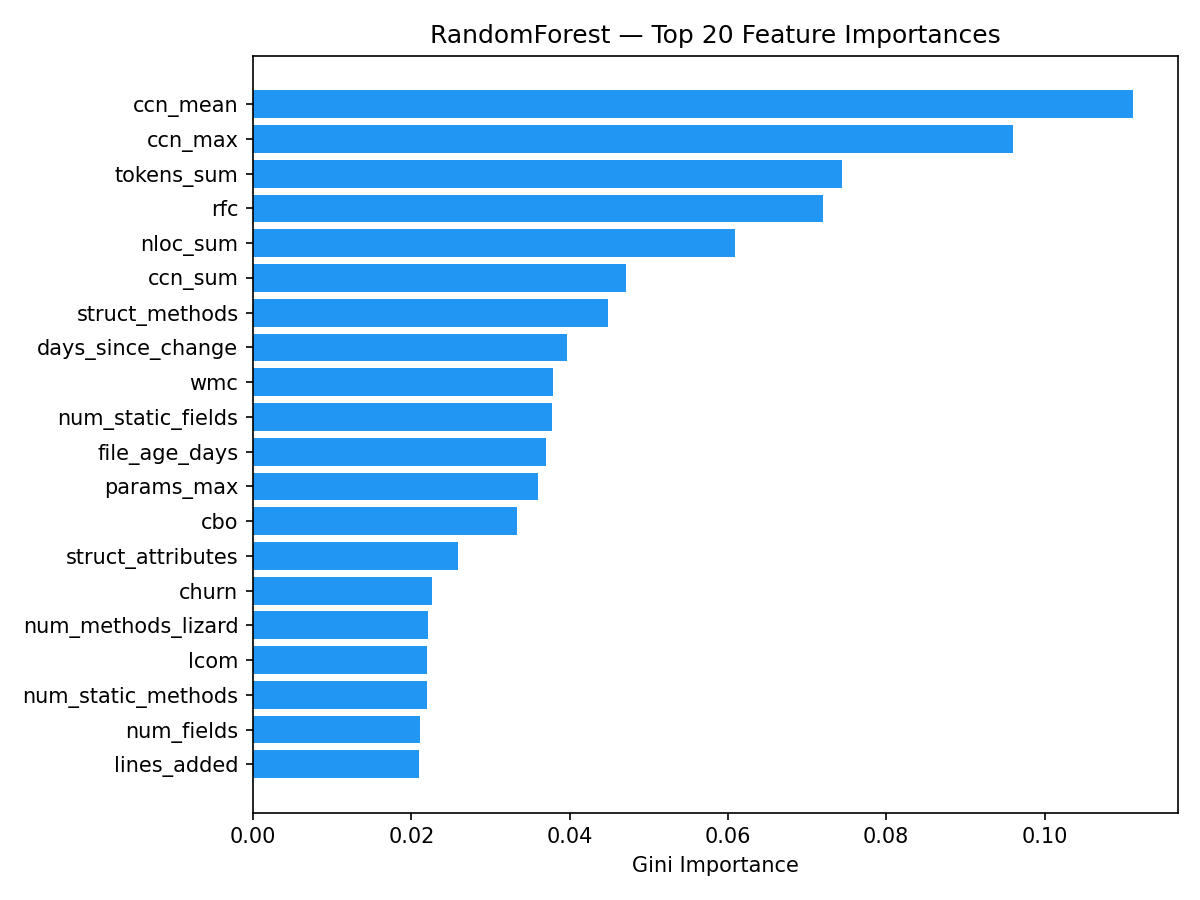
\includegraphics[width=0.8\textwidth]{figuras/feature_importance_rf.png}
\caption{Importância das \textit{features} (\textit{Random Forest}, Gini).}
\label{fig:imp}
\end{figure}

% =====================================================================
\section{Conclusão}
% =====================================================================

Construiu-se um \textit{pipeline} estático e reprodutível que extrai métricas de
qualidade e de segurança de 10 repositórios Java da NSA e treina modelos para
prever arquivos propensos a risco de segurança, com as \textit{features}
amarradas às características da ISO/IEC~25010. Os resultados (ROC-AUC até 0,82)
indicam que métricas de \emph{Manutenibilidade} carregam sinal preditivo sobre
\emph{Segurança}, embora a classificação precisa seja difícil devido ao forte
desbalanceamento.

\textbf{Limitações:} (i)~\emph{Safety} não foi medida (nenhuma ferramenta o
faz) e é tratada conceitualmente; (ii)~cobertura de testes está ausente, pois
não houve execução; (iii)~a SCA cobre sobretudo dependências diretas (transitivas
parciais sem \textit{build}); (iv)~o rótulo de segurança é uma aproximação por
SAST de fonte, sujeita a falsos positivos/negativos; (v)~sem \textit{bytecode},
o SonarQube não seria oráculo de segurança Java --- por isso o alvo veio do
Semgrep; (vi)~a homogeneidade do ecossistema \emph{DataWave} (quatro
repositórios) afeta a validade externa.

\textbf{Trabalhos futuros:} reforçar o rótulo com CodeQL (\texttt{build-mode:
none}); ampliar a amostra para organizações distintas; e explorar limiares de
decisão calibrados por custo para melhorar Recall sob desbalanceamento.

\section*{Disponibilidade}
\textit{Scripts}, \textit{dataset} em nível de arquivo, dicionário de dados e
versões das ferramentas estão documentados no repositório do projeto
(\texttt{TOOLS\_VERSIONS.md}, \texttt{RUN\_LOG.md}), atendendo ao requisito de
reprodutibilidade.

\bibliographystyle{sbc}
\bibliography{referencias}

\end{document}
